\documentclass[12pt, letterpaper]{../assignment}
\usepackage{graphicx}
\usepackage{courier}
\usepackage{minted}
\usepackage{amsmath}
\usepackage{commath}
\usepackage{amssymb}
\usepackage{amsfonts} 
\usepackage{cancel}
\usepackage{enumitem}
\usepackage{array}

\usepackage{tikz}
\usetikzlibrary{shapes,arrows,positioning}

\usemintedstyle{monokai}
\oddsidemargin = 0pt
\exercisesheet{Module 10}{Practice Assignment}
\student{Austin Barrilleaux}
\courselabel{EN 525.609}
\semester{Fall 2023}
\usepackage[backend=bibtex,style=numeric,sorting=none]{biblatex}
\bibliography{reference}
\usepackage{color}
\definecolor{light-gray}{rgb}{0.2,0.2,0.2}
\setminted{bgcolor=light-gray}
\setlength{\parindent}{0pt}

\makeatletter
\patchcmd{\minted@colorbg}{\noindent}{\medskip\noindent}{}{}
\apptocmd{\endminted@colorbg}{\par\medskip}{}{}
\makeatother

\begin{document}
\subsection*{Problem 1}
% \subsubsection*{Solve the following practice problems in the 9th edition textbook.\\
% \begin{itemize}
%     \item Chapter 8:
%     \begin{itemize}
%         \item 8-1
%         \item 8-5
%     \end{itemize}
% \end{itemize}}

\subsubsection*{Solve problem 8-19 in the 9th Edition textbook.\\
\begin{itemize}
    \item Given the following CE:\ \ $ \mathbf{s(s^3 + 2s^2 + s + 1) + K(s^2 + s + 1) = 0} $
    \item (a) Hand-sketch the polar plot as discussed in Module 10 and apply the Nyquist criterion to determine the values of K for system stability.
    \item (b) Check the answers by means of the Routh-Hurwitz criterion.
\end{itemize}}

From the above CE:

$$ 1 + G(s)H(s) = s(s^3 + 2s^2 + s + 1) + K(s^2 + s + 1) = 0 $$

Putting this into the form:

$$ 1 + G(s)H(s) = 1+ L(s) $$

We find that $L(s)$:

$$ L(s) = \frac{K(s^2 + s + 1)}{s(s^3 + 2s^2 + s + 1)} $$

Or:

$$ L(j\omega) = \frac{K\,\left(-\omega ^2+\omega j+1\right)}{\omega ^4- 2\omega ^3j-\omega ^2+\omega j} $$

Simplifying to:

\begin{equation*}
    \begin{aligned}
    L(j\omega) &= \frac{K\,\left((1-\omega ^2)+\omega j\right)}{(\omega ^4-\omega ^2)+j(\omega- 2\omega ^3)} \\
    &=  \frac{K\,\left((1-\omega ^2)+\omega j\right)}{(\omega ^4-\omega ^2)+j(\omega- 2\omega ^3)} \\
    &=  \frac{K\,\left((1-\omega ^2)+\omega j\right)}{(\omega ^4-\omega ^2)+j(\omega- 2\omega ^3)}
    \left(\frac{(\omega ^4-\omega ^2)-j(\omega- 2\omega ^3)}{(\omega ^4-\omega ^2)-j(\omega- 2\omega ^3)}\right) \\
    &=  \frac{K\left(-\omega ^6+ j(-\omega ^5 +2 \omega ^3 -\omega  )\right)}{(\omega ^4-\omega ^2)+(\omega- 2\omega ^3)}
    \end{aligned}
\end{equation*}

The Magnitude of $L(j\omega)$ is:

$$ |L(j\omega)| = \left|\frac{K\left(-\omega ^6+ j(-\omega ^5 +2 \omega ^3 -\omega  )\right)}{(\omega ^4-\omega ^2)+(\omega- 2\omega ^3)} \right| $$

The Angle of $L(j\omega)$ is:

$$ \angle L(j\omega) = \tan^{-1}\left( \frac{-\omega ^5 +2 \omega ^3 -\omega  }{-\omega ^6}\right) = 180^\circ - \tan^{-1} \left(\frac{-\omega ^4 +2 \omega ^2 - 1 }{\omega ^5}\right) $$

From this, we can determine the following, evaluating the limit as $\omega = 0$:

$$ \lim_{\omega \to 0} L(j\omega) = \infty   $$

$$ \lim_{\omega \to 0} \angle L(j\omega) = 180 -\tan^{-1}\left(\frac{-1}{0}\right) = 270^\circ = -90^\circ $$

From this, we can determine the following, evaluating the limit as $\omega = \infty$:

$$ \lim_{\omega \to \infty} L(j\omega) = 0   $$

$$ \lim_{\omega \to \infty} \angle L(j\omega) = 180 -\tan^{-1}\left(\frac{-1}{\infty}\right) = 180^\circ $$

Finding intersection of the locus with the real axis via: $\text{Im}[L(j\omega)]=0$:

$$ -\omega ^5 +2 \omega ^3 -\omega = 0 \ \ \ \rightarrow \ \ \ \omega ^4 -2 \omega ^2 +1 = 0 $$

This can be factored to:

$$ (\omega ^2 - 1)^2 = 0 \ \ \ \rightarrow \ \ \ \omega = \pm 1\ \text{rad/s}$$

Substituting, $L(j\omega)$:

$$ |L(j1)| = \frac{K(s^2 + s + 1)}{(s^4 + 2s^3 + s^2 + s)} = \frac{K(-1 + j + 1)}{(1 - 2j -1 + j)} = K\frac{j}{-j} = -K $$

$$ \angle L(j1) = \angle \frac{K(-1 + j + 1)}{(1 - 2j -1 + j)} = 180 -\tan^{-1}\left(\frac{0}{-1}\right) = 180^\circ  $$

Plotting this, we get a plot that looks something like:

\begin{figure}[H]
    \centering
    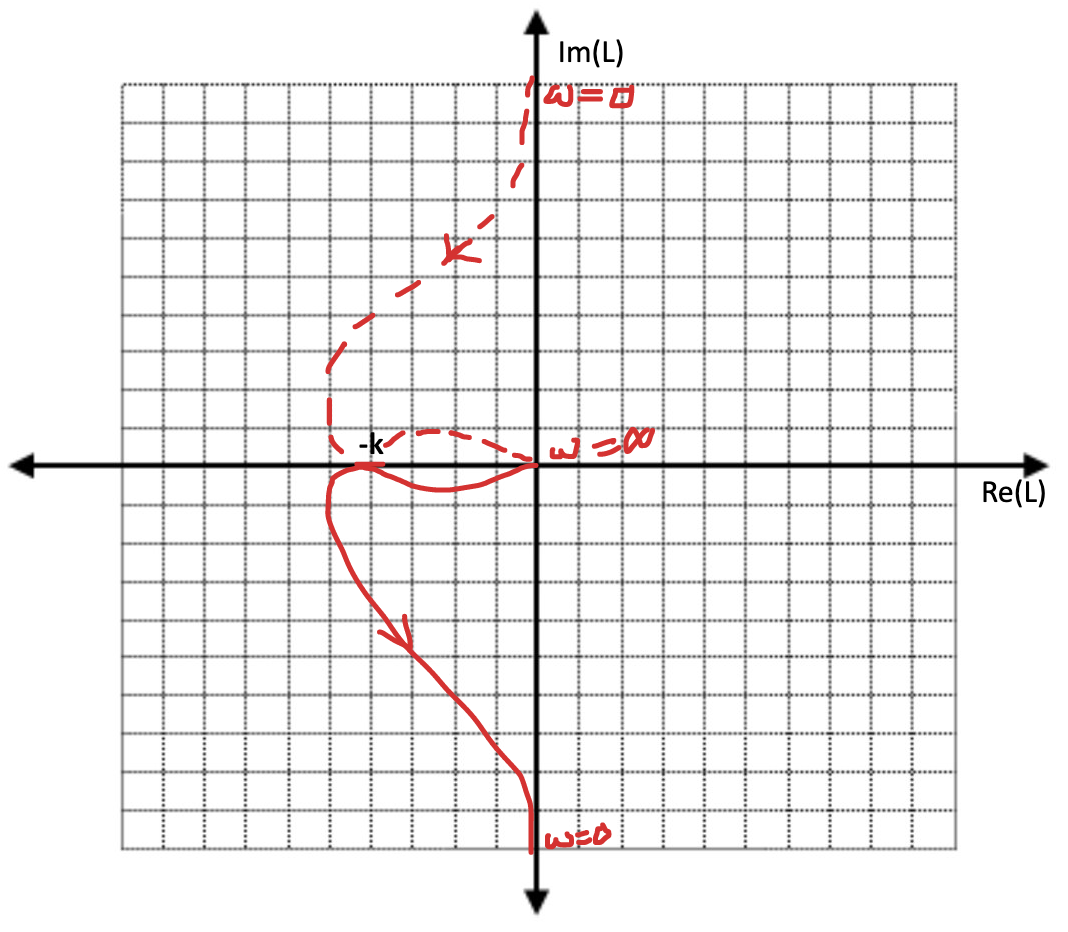
\includegraphics[width=0.5\linewidth]{./figures/PolarPlot1.png}
    % \caption{Polar Plot}
    \label{fig:pp1}
 \end{figure}

Applying the Nyquist Stability Criterion:

 $$ N=Z-P $$
 
Where:\\
$N =$ number of encirclements of the $(-1, j0)$ point made by the $L(s)$ plot.\\
$Z =$ number of zeros of $1+L(s)$ that are inside the Nyquist path, that is, the right-half s-plane.\\
$P =$ number of poles of $1+L(s)$ that are inside the Nyquist path, that is, the right-half s-plane.
(Notice that the poles of $1 +L(s)$ are the same as that of $L(s)$.)\\

There are zero poles of $L(s)$ in the RHP (MATLAB: $\texttt{roots([1 2 1 1 0])} = 0,- 0.1226 \pm 0.7449j,-1.7549$), so $P = 0$.
For the system to be stable ($Z=0$),
there must be zero encirclements of the $(-1, j0)$ point ($N = 0$.)

As stated above, the Phase Angle of $L(j\omega)$ is:

$$ \angle L(j\omega) = \tan^{-1}\left( \frac{-\omega ^5 +2 \omega ^3 -\omega  }{-\omega ^6}\right) $$

In the event that $K$ is negative, the negative sign would impact this angle:

$$ \angle L(j\omega) = \tan^{-1}\left( \frac{\omega ^5 -2 \omega ^3 +\omega  }{-\omega ^6}\right) $$

So when evaluating the angle as $\omega \rightarrow 0$,
the angle would be positive $90^\circ$ instead of $-90^\circ$. In this case, the $(-1, j0)$ would be enclosed,
so the system would be unstable since $Z$ would not be zero.

\begin{answer}
Therefor, the \textbf{system is stable when} $K > 0$, and the \textbf{system is unstable when} $K < 0$. If $K=1$, the contour would lie on the point $(-1, j0)$, so the \textbf{system would be marginally stable}.
\end{answer}


Evaluating with Routh-Hurwitz, we get the following table:

$$ \begin{array}{c|ccc} s^4 & 1 & K+1 & K\\ s^3 & 2 & K+1 & 0\\ s^2 & \frac{K+1}{2} & K & 0\\ s^1 & \frac{K^2-2K+1}{K+1} & 0 & 0\\ s^0 & K & 0 & 0 \end{array}$$

\begin{answer}
This reinforces the above conclusion.
The \textbf{system is stable when} $K > 0$, and \textbf{unstable when} $K < 0$.
\end{answer}

The leftmost column of $s^1$ equates to:

$$ \frac{K^2-2K+1}{K+1} = \frac{(K-1)^2}{K+1} $$

Set equal to zero:

$$ \frac{(K-1)^2}{K+1} = 0 $$

\begin{answer}
We see that when $K = 1$, we get a row of all zeros implying complex poles on the imaginary axis. In this case, \textbf{the system is marginally stable.}
\end{answer}

\subsection*{Problem 2}
\subsubsection*{Consider the open loop transfer function, below, which is placed in a unity-feedback configuration:
$$ \mathbf{G(s) = \frac{5(s-2)}{s (s+1)(s-1)} } $$
\begin{itemize}
    \item (a) Draw the entire polar plot of this system.
    \item (b) Considering the portion of the polar plot from
    $\mathbf{\omega=+\infty}$ to $\mathbf{\omega=0+}$,
    apply the Nyquist criterion to determine the stability of the system.
    If the system is unstable, determine the number of closed loop poles in the RHP.
\end{itemize}}


The open loop transfer function in question can be written as:

$$ G(j\omega) = \frac{5(j\omega-2)}{(j\omega)^3 - j\omega} $$

Simplifying to:

\begin{equation*}
    \begin{aligned}
        G(j\omega) &= \frac{5(j\omega-2)}{(j\omega)^3 - j\omega}\\
                   &= \frac{5(j\omega-2)}{-j \omega^3 - j\omega}\\
                   &= \frac{5(j\omega-2)}{-j (\omega^3 + \omega)}\\
                   &= \frac{5(j\omega-2)}{-j (\omega^3 + \omega)}
                      \left(\frac{j(\omega^3 + \omega)}{j(\omega^3 + \omega)}\right)\\
                   &= \frac{-5 \omega ^2 (\omega ^2 + 1) -10 j \omega (\omega ^2 + 1)}{(\omega^3 + \omega)^2}
    \end{aligned}
\end{equation*}

The Magnitude of $G(j\omega)$ is:

$$ |G(j\omega)| = \left|\frac{-5 \omega (\omega ^2 + 1) -10 j (\omega ^2 + 1)}{\omega(\omega^2 + 1)^2} \right| $$

The Angle of $G(j\omega)$ is:

$$ \angle G(j\omega) = \tan^{-1}\left( \frac{10 \omega (\omega ^2 + 1)}{5 \omega ^2 (\omega ^2 + 1)}\right) = \tan^{-1} \left(\frac{2}{\omega}\right) $$

From this, we can determine the following evaluating the limit as $\omega = 0$:

$$ \lim_{\omega \to 0} L(j\omega) = \infty   $$

$$ \lim_{\omega \to 0} \angle L(j\omega) = \tan^{-1} \left(\frac{2}{0}\right) = 90^\circ $$

From this, we can determine the following evaluating the limit as $\omega = \infty$:

$$ \lim_{\omega \to \infty} L(j\omega) = 0  $$

$$ \lim_{\omega \to 0} \angle L(j\omega) = \tan^{-1} \left(\frac{2}{\infty}\right) = 0^\circ $$

We can check for a real axis intersection:

$$ 10 (\omega ^2 + 1) = 0$$

Which simplifies to:

$$ \omega ^2 = -1 \ \ \rightarrow \ \ \omega = \pm j $$

No real axis crossing exists:
\\\\
We can check for an imaginary axis intersection:

$$ 5 \omega (\omega ^2 + 1) = 0$$

Which simplifies to:

$$ \omega ^2 = -1 \ \ \rightarrow \ \ \omega = \pm j $$

No imaginary axis crossing exists:
\\\\
Using this information, the polar plot will look like the following:

\begin{figure}[H]
    \centering
    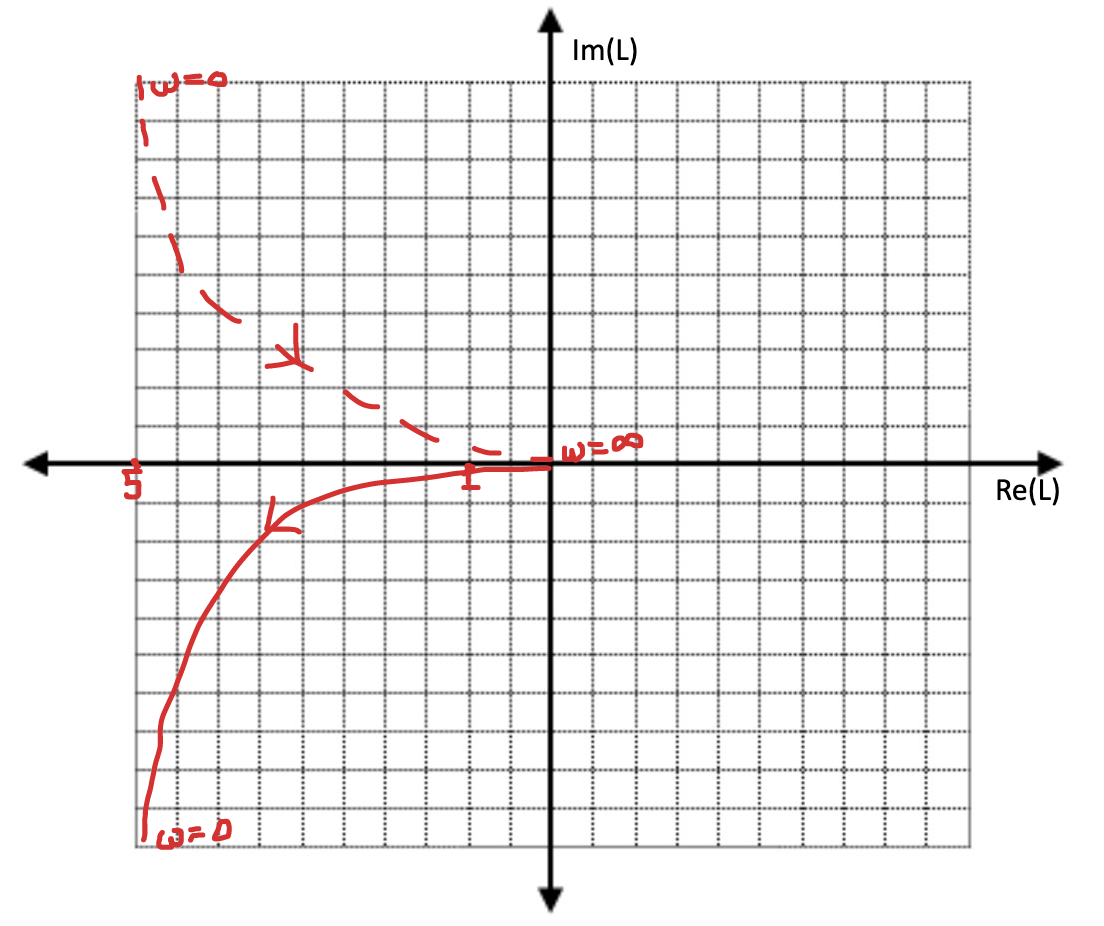
\includegraphics[width=0.5\linewidth]{./figures/PolarPlot2.png}
  %  \caption{Polar Plot}
    \label{fig:pp2}
 \end{figure}
  
Applying the Nyquist Stability Criterion:

$$ N=Z-P $$

Where:\\
$N =$ number of encirclements of the $(-1, j0)$ point made by the $L(s)$ plot.\\
$Z =$ number of zeros of $1+L(s)$ that are inside the Nyquist path, that is, the right-half s-plane.\\
$P =$ number of poles of $1+L(s)$ that are inside the Nyquist path, that is, the right-half s-plane.
(Notice that the poles of $1 +L(s)$ are the same as that of $L(s)$.)\\

There is one open loop pole in the RHP, so $P = 1$.
(The open loop transfer function is not stable.)
Looking at the Polar Plot, $(-1, j0)$ is not enclosed by the contour, so $N = 0$.
Solving for $Z$:

$$ Z = N+P = 0+1 = 1 $$

\begin{answer}
    Since $Z \ne 0 $, the \textbf{closed loop system is not stable!}.
    There is \textbf{1 closed loop pole in the RHP.}
\end{answer}



% \color{white}
% \hspace*{6em}\inputminted[frame=leftline,fontsize=\footnotesize]{matlab}
% {./matlab/Problem_5_18.m}
% \color{black}

% \begin{figure}[H]
%     \centering
%     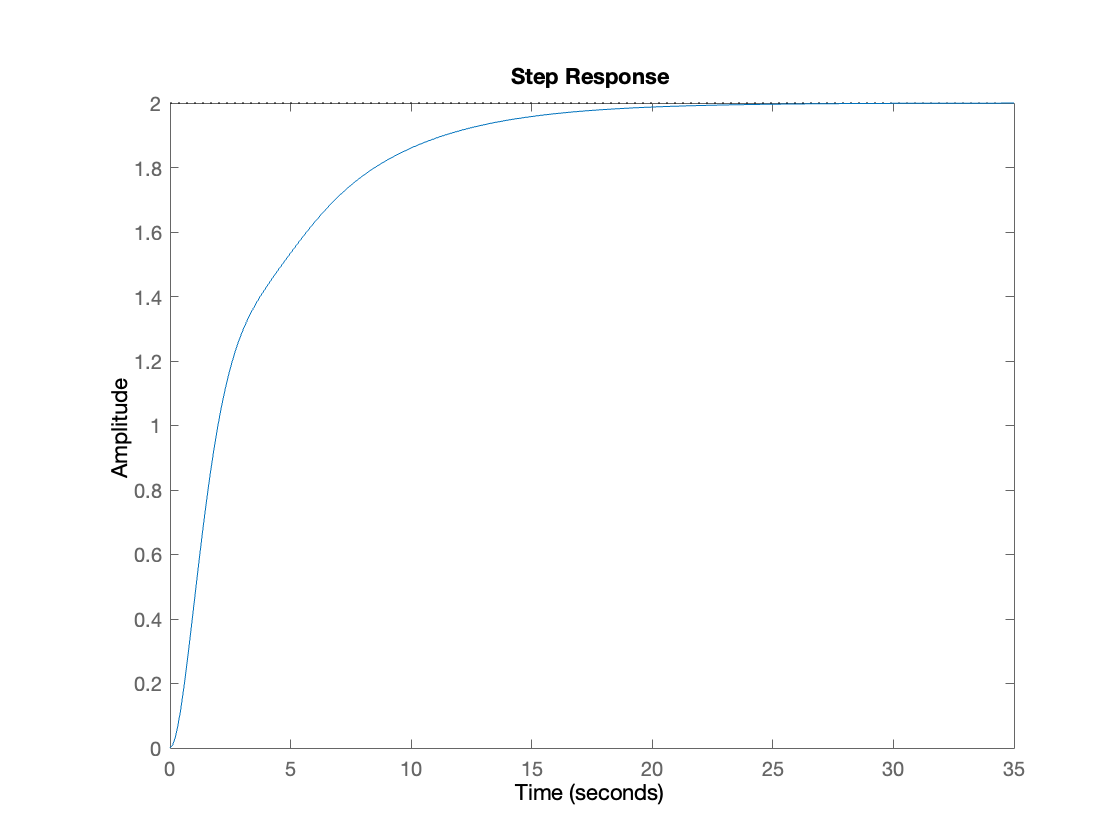
\includegraphics[width=0.7\linewidth]{./figures/step_response.png}
%     \caption{Step Response}
%     \label{fig:step}
%  \end{figure}



\end{document}

